\section{Verifying calibration}
\label{sec:verifying_calibration}

\newcommand{\pluginEst}[0]{\ensuremath{\hat{E}_{pl}^2}}
\newcommand{\cancelEst}[0]{\ensuremath{\hat{E}^2}}
\newcommand{\ltwoerror}[0]{\ensuremath{{\hat{E}^*}^2}}
\newcommand{\piSmallBound}[0]{\ensuremath{\frac{12}{n}\log{\frac{2B}{\delta}}}}

\pl{isn't a easier way of saying this, we can only estimate the calibration error of binned calibrators? as we showed in previous section}
If a model outputs values from some finite set $S$,\footnote{The model can choose the set $S$.} and the probability of outputting each value $s \in S$ is not too small, then we can estimate its calibration error. The plugin estimator \pl{explain this (make simple things simple)} used in past work requires samples proportional to the number of model outputs $|S|$. Instead, we introduce the \emph{cancelling} estimator that requires samples proportional to $\sqrt{|S|}$. At a high level, the cancelling estimator leverages cancellation of error terms across different bins.

\pl{why not use $B$ instead of $|S|$?}
\pl{I guess there's a subtlety that here, we're talking about specific values not bins...}

% We prove these finite sample guarantees (Theorem~\ref{thm:final-ours}), and show experimental evidence that our estimators approximate the calibration error better. We also show, experimentally, that using a better estimator allows us to pick out better models.

The plugin estimator directly estimates each term in the $\ell_2^2$ calibration error from samples~\cite{nguyen2015posterior, hendrycks2019anomaly, kuleshov2015calibrated, hendrycks2019pretraining}. Suppose we wish to measure the calibration error of a model $f : \mathcal{X} \to S$ where $S \subseteq [0, 1]$. Order the elements in $S$: $s_1 < s_2 < \dots < s_B$, where $B = |S|$ denotes the number of model outputs. Suppose we get an evaluation set $T_n = \{(x_1, y_1), \dots, (x_n, y_n)\}$ sampled i.i.d. from $P(X, Y)$.

\pl{notationally, you can index directly using $s$ instead of $i$ to save one level of indirection}

\begin{restatable}[Plugin estimator]{definition}{pluginDfn}
\label{dfn:plugin-estimator}
\pl{English: define $\hat y_i$ to be the empirical average for the $i$-th score}
  Let $L_i = \{ y_j \; | \; (x_j, y_j) \in T_n\wedge f(x_j) = s_i \}$ \pl{background this} denote the label values where the model outputs $s_i$.

We estimate $E[Y | f(X) = s_i]$ as:
\[ \hat{y_i} = \sum_{y \in L_i} \frac{y}{|L_i|} \] 
  \pl{English: define $\hat p_i$ to be the actual average for the $i$-th score}
We estimate $P(f(X) = s_i)$ by:
\[ \hat{p_i} = \frac{|L_i|}{n} \]
  Then the plugin estimator for the $\ell_2^2$ error is \pl{the weighted squared difference between the two}:
  \pl{$b$ should be upper case (see throughout)}
  \pl{but if you use the notation, then you have
  \[ \mathcal{E}_\text{plugin} = \sum_{s \in S} \hat{p_s} (s - \hat{y_s})^2 \]
  }
\[ \pluginEst{} = \sum_{i=1}^B \hat{p_i} (s_i - \hat{y_i})^2 \]
\end{restatable}
\pl{can we just use $L^2$ for this whole paper?}

We now define our improved cancelling estimator. The key insight is that the plugin estimate of the error in each bin, $(s_i - \hat{y_i})^2$ is biased. By debiasing these estimates we get cancellations across bins.

\pl{this formula is a bit out of nowhere; saying 'debiasing' is helpful, but can you actually say the criteria more formally and declaratively?}
\begin{restatable}[Cancelling estimator]{definition}{cancelingDfn}
The cancelling estimator for the $\ell_2^2$ error is:
\[ \hat{E}^2 = \sum_{i=1}^b \hat{p_i} \Big[ (s_i - \hat{y_i})^2 - \frac{\hat{y_i}(1 - \hat{y_i})}{\hat{p_i}n-1} \Big] \]
\end{restatable}

The main results are that to check if the $\ell_2^2$ calibration error of a model is $\leq \epsilon^2$, the plugin estimator requires $\Theta(\frac{B}{\epsilon^2})$ samples (Theorem~\ref{thm:final-plugin}) while our estimator requires $\theta(\frac{\sqrt{B}}{\epsilon^2})$ samples (Theorem~\ref{thm:final-ours}). We begin by giving a bound on the error of the plugin estimator.

\begin{restatable}{theorem}{pluginBound}
\label{thm:plugin-bound}
Let $p_i = P(f(X) = s_i)$ and suppose $p_i > \piSmallBound{}$ for all $i$. Let $c(n)$ be defined as:
\[ c(n) = \sqrt{\frac{3}{n \min p_i} \log{\frac{2B}{\delta}}} \]
Then for the plugin estimator, with probability at least $1 - 3\delta$,
\[ | \hat{E_{pl}}^2 - {E^*}^2 | \leq c(n){E^*}^2 + \sqrt{\frac{2(1+c(n)){E^*}^2}{n} \log{\frac{2}{\delta}}} + \frac{B}{2n} \log{\frac{2B}{\delta}} \]
\end{restatable}

Typically, we are interested in checking if our model has calibration error $\leq \epsilon$ \pl{but this is not what we actually show due to $r$}. \pl{say that the next theorem studies this} In other words, we are given $\epsilon, \delta > 0$ and effect size $0 < r < 1$ \pl{where did effect size come from? I think all of this should be set up as what we want before doing the analysis}. If the calibration error is $> \epsilon$, then with probability at least $1 - \delta$ we should output that it is not calibrated \pl{be more precise}. If the calibration error is $< r\epsilon$, then with probability at least $1 - \delta$, we should output that the model is calibrated.

\begin{restatable}[Plugin bound]{theorem}{finalPlugin}
\label{thm:final-plugin}
  Suppose \pl{use English} $\forall i.\;p_i \geq \frac{1}{2B}$ and $n = \Theta(\frac{B}{\epsilon^2})$ ignoring $\log$ factors. Then the plugin estimator can check if ${E^*}^2 \leq \epsilon^2$ with failure probability $\delta$, and constant effect size $0 < r < 1$. 
\end{restatable}

Another way of thinking about this is that if $n = \Theta(\frac{B}{{E^*}^2})$ then \pl{English} $r {E^*}^2 \leq \hat{E_{pl}}^2 \leq (1+r){E^*}^2$.

\pl{should be separate subsection}
Next we bound the error of the cancelling estimator.

% \subsection{Analysis of our estimator}

\begin{restatable}{theorem}{cancelingBound}
\label{thm:our-bound}
Let $p_i = P(f(X) = s_i)$ and suppose $p_i > \piSmallBound{}$ for all $i$. Let $c(n)$ be as defined in Theorem~\ref{thm:plugin-bound}.
Then for the cancelling estimator, with probability at least $1 - 4\delta$,
\[ | \hat{E}^2 - {E^*}^2 | \leq c(n){E^*}^2 + \sqrt{\frac{2(1+c(n)){E^*}^2}{n} \log{\frac{2}{\delta}}} + \frac{3\sqrt{B}}{n} \log{\frac{n}{\delta}} + \frac{\delta}{n}\]
\end{restatable}


\begin{restatable}[Cancelling bound]{theorem}{finalCanceling}
\label{thm:final-ours}
Suppose $\forall i.\;p_i \geq \frac{1}{2B}$ and $n = \Theta(B+\frac{\sqrt{B}}{\epsilon^2})$ ignoring $\log$ factors. Then the cancelling estimator can check if ${E^*}^2 \leq \epsilon^2$ with failure probability $\delta$ and constant effect size $r$. 
\end{restatable}
\tm{may be good to explain what's the dominating term. How to interpret the bound ---}
\pl{provide a few sentences for proof sketch - at least the highlights - standard concentration or anything new? what's the hard part?}

\subsection{Experiments}

We ran experiments on CIFAR-10 and Imagenet to compare the practical performance of the cancelling estimator and the plugin estimator. We split the validation set \pl{how big?} into two chunks $C_1$ \pl{maybe give these more meaningful names with subscripts? anyway, put them behind macros} and $C_2$ \pl{what sizes}. We use $C_1$ to re-calibrate and discretize a trained model using $B = 100$ bins. For varying values of $n$, we sample $n$ points, with replacement, from $C_2$, and estimate the calibration error using the cancelling estimator and the plugin estimator. We then compute the squared deviation of these estimates from the calibration error measured on the entire chunk $C_2$. We repeat this 1,000 times to get the mean squared deviation and confidence intervals. The results are in Figure~\ref{fig:mse_estimators}. \pl{always say what the result is: Figure shows that...}
In the Appendix, we include results for ImageNet, ablations on $B$, and we visualize the histogram of the deviations.

\pl{say explicitly that we never say 'not calibrated'; there's a disconnect between the theory, which requires $r$ and $\epsilon$ and what we're doing here}

We also run a multi-class calibration experiment on CIFAR-10 to show that our estimator allows us to select models with a better \pl{lower} Brier \pl{should we just say MSE everywhere? just be consistent since you defined MSE at the beginning} score subject to a given calibration constraint. As before, we split the validation set into $C_1$ and $C_2$. On $C_2$, we estimate the calibration error using the plugin and cancelling estimators and use 100 Bootstrap resamples to compute a 90\% upper confidence bound on the estimate. We compute the Brier scores and the upper bounds on the calibration error for $B = 10, 15, \cdots, 100$ and show the Pareto curve in Figure~\ref{fig:mse_vs_ce_estimators}. The results show that for any desired calibration error, the cancelling estimator enables us to pick out models with a better Brier score.

\begin{figure}
  \centering
  \centering
     \begin{subfigure}[b]{0.45\textwidth}
         \centering
         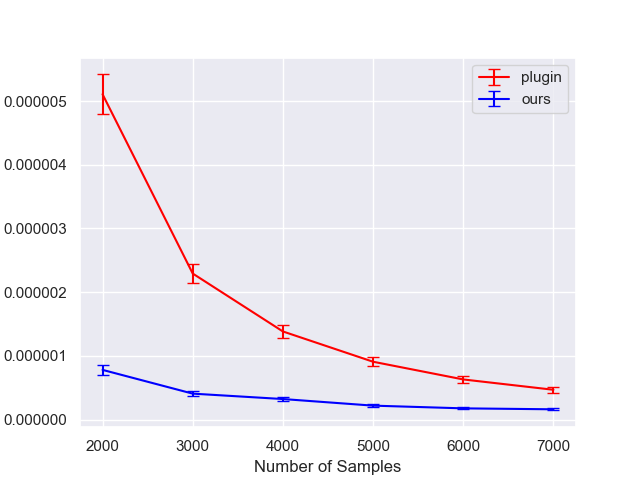
\includegraphics[width=\textwidth]{mse_estimator_100_bins.png}
         \caption{Mean-squared errors of estimates.
         \pl{s/ours/canceling}
         \pl{Number of samples of what - relate to notation in text}
         \pl{label y-axis}
         }
         \label{fig:mse_estimators}
     \end{subfigure}
     \hfill
     \begin{subfigure}[b]{0.45\textwidth}
         \centering
         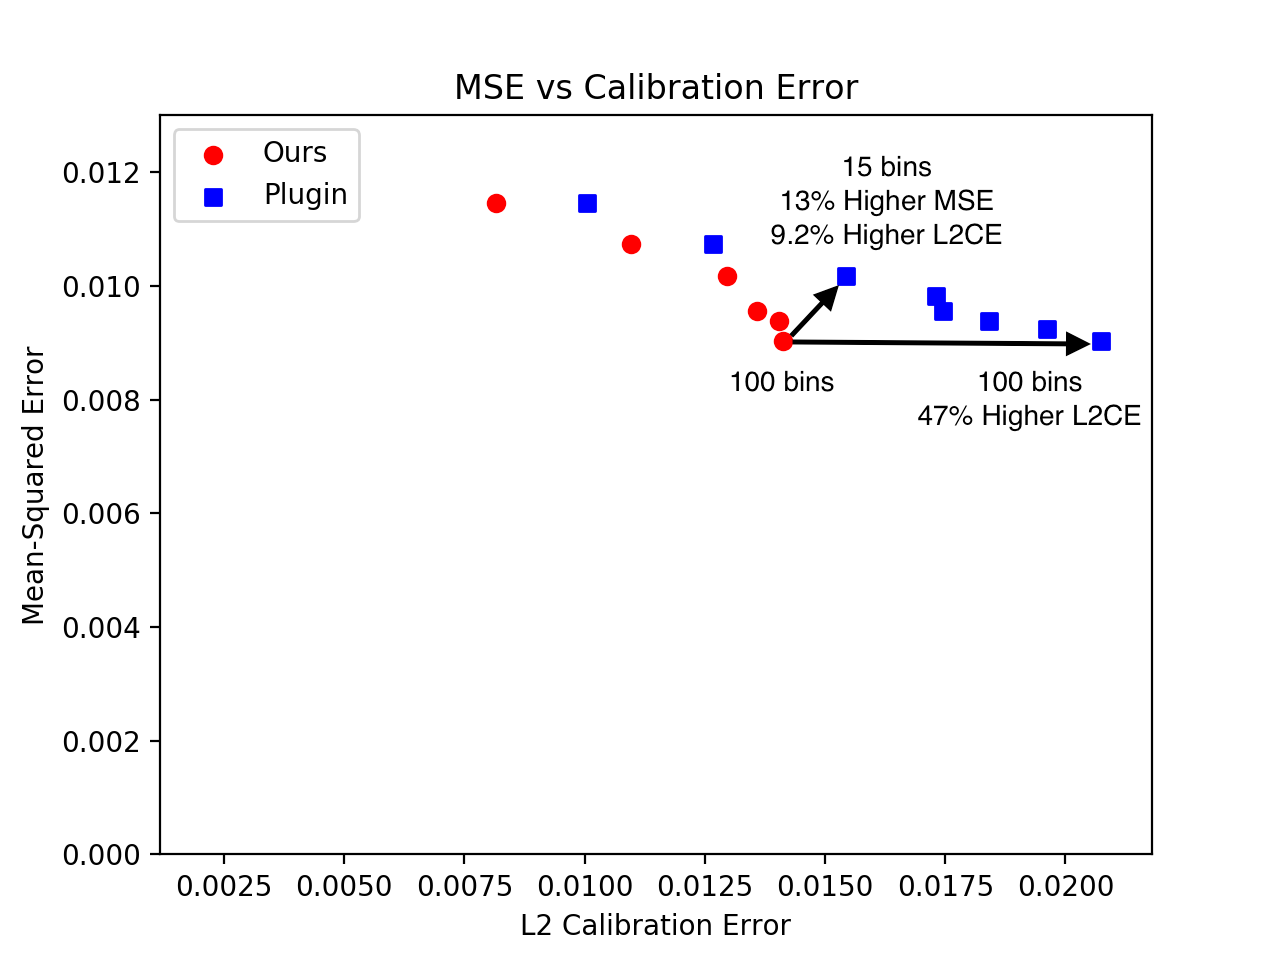
\includegraphics[width=\textwidth]{mse_vs_verified_error_plugin_vs_ours.png}
         \caption{Brier score vs calibration error.
         \pl{be consistent with MSE/Brier}
         \pl{make text larger by reducing the xrange and yrange}
         }
         \label{fig:mse_vs_ce_estimators}
     \end{subfigure}
  \caption{
    (\textbf{Left}) Mean-squared errors of cancelling and plugin estimators on a recalibrated VGG-net model on CIFAR-10 with $90\%$ confidence intervals (lower values better). Our estimator is closer to the ground truth \pl{what's ground truth? 0 on the y-axis?}.
  (\textbf{Right}) Plot of Brier scores against upper bounds \pl{90\% confidence bounds or something?} on the calibration error computed by our estimator and the plugin estimator, when we vary the number of bins $B$. For a given calibration error, our estimator enables us to choose models with a better Brier score. If we want a model with $\ell_2$ calibration error less than 0.015, the cancelling estimator tells us we can confidently use 100 bins, while relying on the plugin estimator only lets us use 15 bins and incurs a 13\% higher Brier score.
  \pl{I find it awkward that you have MSE (which is squared) plotted against calibration error (non-squared);
  can we just make it RMSE instead?
  }
}
  \label{fig:mse_estimators_bins}
\end{figure}

% This means that our estimator has a substantially better dependency on the number of outputs of the model.

% \begin{corollary}
% \label{cor:final-ours}
% Using our estimator $\hat{E}$, if $n = \Theta(kb + \frac{\sqrt{b}}{\epsilon^2})$ ignoring $\log$ factors, we can check if $|{E^*} | \leq \epsilon$ with significance and power $\delta$, and constant effect size $r$. 
% \end{corollary}
